\chapter{El corazón y la circulación}\label{ch:g7:heart-and-circulation}

El \cref{ch:g4:heart-and-blood} presentó la bomba y sus rondas de
reparto; desde entonces la \omterm{prop:g4:journey-of-food:absorb}{sangre} ha ido acumulando responsabilidades
--- \omterm{def:g7:digestion-and-nutrients:families}{nutrientes} en las \omterm{prop:g7:digestion-and-nutrients:absorption}{vellosidades}
(\cref{prop:g7:digestion-and-nutrients:absorption}), \omterm{def:g7:what-is-respiration:respiration}{oxígeno} en los
\omterm{def:g7:lungs-and-gas-exchange:alveoli}{alvéolos} (\cref{prop:g7:lungs-and-gas-exchange:numbers}) y facturas en
todos los \omterm{def:g3:bones-and-muscles:muscle}{músculos} que trabajan
(\cref{prop:g7:organs-at-work:bill}). Toca cartografiar como es debido
la red de carreteras: las cuatro habitaciones del \omterm{def:g4:heart-and-blood:heart}{corazón}, los dos
circuitos y las tres clases de vaso.

\section{Las cuatro habitaciones del corazón}

\begin{definition}[Aurículas y ventrículos]\label{def:g7:heart-and-circulation:rooms}
Cada uno de los dos lados del \omterm{def:g4:heart-and-blood:heart}{corazón}
(\cref{def:g4:heart-and-blood:heart}) tiene dos habitaciones: arriba
una \emph{aurícula}\index{aurícula}, que recibe la \omterm{prop:g4:journey-of-food:absorb}{sangre} que llega, y
abajo un \emph{ventrículo}\index{ventrículo} --- la sala de bombeo de
paredes gruesas --- que la empuja hacia fuera. Entre ellas y más allá,
unas \emph{válvulas}\index{válvula (corazón)} --- puertas de un solo
sentido --- se cierran de golpe detrás de cada oleada; sus golpes por
parejas son exactamente el ``pum-pum'' que oye un fonendoscopio (o una
\omterm{def:g1:the-five-senses:sense}{oreja} apoyada en un pecho).
\end{definition}

\begin{proposition}[Un latido, por orden]\label{prop:g7:heart-and-circulation:beat}
Cada \omterm{def:g4:heart-and-blood:heart}{latido} recorre la misma secuencia en los dos lados a la vez: las
\omterm{def:g7:heart-and-circulation:rooms}{aurículas} se contraen y acaban de llenar los \omterm{def:g7:heart-and-circulation:rooms}{ventrículos}; los
\omterm{def:g7:heart-and-circulation:rooms}{ventrículos} se contraen y empujan la \omterm{prop:g4:journey-of-food:absorb}{sangre} hacia fuera --- el lado
derecho hacia los \omterm{def:g7:how-animals-breathe:four}{pulmones} y el izquierdo hacia el cuerpo --- mientras
las \omterm{def:g7:heart-and-circulation:rooms}{válvulas} de entrada dan su portazo (pum); los \omterm{def:g7:heart-and-circulation:rooms}{ventrículos} se
relajan, las \omterm{def:g7:heart-and-circulation:rooms}{válvulas} de salida dan el suyo (pum) y las habitaciones
se vuelven a llenar. Y otra vez, $100000$ veces al día
(\cref{rem:g4:heart-and-blood:rest}).
\end{proposition}
\admitted

\section{Dos circuitos, tres vasos}

\begin{definition}[La circulación doble]\label{def:g7:heart-and-circulation:double}
La red de carreteras de la \omterm{prop:g4:journey-of-food:absorb}{sangre} son dos bucles que pasan por una sola
bomba (los dos lados de la
\cref{def:g4:heart-and-blood:heart}, ahora como circuitos):
\begin{itemize}
  \item el \emph{circuito pulmonar}: \omterm{def:g7:heart-and-circulation:rooms}{ventrículo} derecho $\rightarrow$
        \omterm{def:g7:how-animals-breathe:four}{pulmones} (carga \omterm{def:g7:what-is-respiration:respiration}{oxígeno}, descarga \omterm{def:g7:what-is-respiration:respiration}{dióxido de carbono})
        $\rightarrow$ \omterm{def:g7:heart-and-circulation:rooms}{aurícula} izquierda;
  \item el \emph{circuito general}: \omterm{def:g7:heart-and-circulation:rooms}{ventrículo} izquierdo $\rightarrow$
        todo el cuerpo (entrega y recoge) $\rightarrow$ \omterm{def:g7:heart-and-circulation:rooms}{aurícula}
        derecha.
\end{itemize}
Todas las gotas van alternando circuitos: \omterm{def:g7:how-animals-breathe:four}{pulmones}, cuerpo, \omterm{def:g7:how-animals-breathe:four}{pulmones},
cuerpo --- que es por lo que el \omterm{def:g7:heart-and-circulation:rooms}{ventrículo} izquierdo, que empuja por el
bucle del cuerpo, mucho mayor, es la habitación de paredes más gruesas
del \omterm{def:g4:heart-and-blood:heart}{corazón}.
\end{definition}

\begin{definition}[Arterias, capilares y venas]\label{def:g7:heart-and-circulation:vessels}
Tres clases de vaso forman cada bucle (los de la
\cref{def:g4:heart-and-blood:vessels}, ahora con nombre):
\begin{itemize}
  \item las \emph{arterias}\index{arteria}: de paredes gruesas y
        elásticas, llevan la \omterm{prop:g4:journey-of-food:absorb}{sangre} \emph{desde} el \omterm{def:g4:heart-and-blood:heart}{corazón} a presión
        --- el \omterm{prop:g4:heart-and-blood:pulse}{pulso} (\cref{prop:g4:heart-and-blood:pulse}) es su
        estiramiento en cada oleada;
  \item los \emph{capilares}\index{capilar}: los \omterm{def:g4:heart-and-blood:vessels}{vasos} finos como un
        \omterm{def:g1:animals-around-us:covering}{pelo} que se cuelan por todos los órganos --- de paredes de una
        \omterm{def:g5:first-look-at-cells:cell}{célula} de grosor, y donde ocurren \emph{todos} los
        intercambios: \omterm{def:g7:lungs-and-gas-exchange:alveoli}{alvéolos}, \omterm{prop:g7:digestion-and-nutrients:absorption}{vellosidades}, \omterm{def:g3:bones-and-muscles:muscle}{músculos}, \omterm{def:g1:the-five-senses:sense}{piel};
  \item las \emph{venas}\index{vena}: anchas, de paredes más finas,
        devuelven la \omterm{prop:g4:journey-of-food:absorb}{sangre} \emph{al} \omterm{def:g4:heart-and-blood:heart}{corazón} a poca presión y con
        \omterm{def:g7:heart-and-circulation:rooms}{válvulas} de un solo sentido propias --- las líneas azuladas de
        la \cref{rem:g4:heart-and-blood:see}.
\end{itemize}
\end{definition}

\begin{omfigure}
\begin{tikzpicture}[scale=0.9]
  % heart center: four rooms
  \draw[thick] (3.8,2.1) rectangle (7.0,3.9);
  \draw[thick] (5.4,2.1) -- (5.4,3.9);
  \draw[thick] (3.8,3.0) -- (7.0,3.0);
  \node[font=\footnotesize, align=center] at (4.6,3.45)
    {aurícula\\ derecha};
  \node[font=\footnotesize, align=center] at (6.2,3.45)
    {aurícula\\ izquierda};
  \node[font=\footnotesize, align=center] at (4.6,2.55)
    {ventrículo\\ derecho};
  \node[font=\footnotesize, align=center] at (6.2,2.55)
    {ventrículo\\ izquierdo};
  % lungs above
  \draw[thick, fill=omDef!8] (4.5,5.2) ellipse (0.75 and 0.6);
  \draw[thick, fill=omDef!8] (6.3,5.2) ellipse (0.75 and 0.6);
  \node[font=\footnotesize] at (5.4,5.95) {los pulmones};
  % body below
  \draw[thick, fill=omProp!8, rounded corners=6pt]
    (3.9,-0.7) rectangle (6.9,0.5);
  \node[font=\footnotesize] at (5.4,-0.1) {todo el cuerpo};
  % lung circuit arrows
  \draw[->, very thick, omDef] (4.9,3.9) .. controls (4.6,4.4)
    .. (4.5,4.6);
  \draw[->, very thick, omThm] (6.3,4.6) .. controls (6.2,4.35)
    .. (5.95,3.92);
  \node[font=\footnotesize, omDef, left] at (4.35,4.45)
    {a cargar oxígeno};
  % body circuit arrows
  \draw[->, very thick, omThm] (5.95,2.1) .. controls (6.3,1.3)
    .. (6.2,0.52);
  \draw[->, very thick, omDef] (4.6,0.52) .. controls (4.5,1.3)
    .. (4.9,2.08);
  \node[font=\footnotesize, omThm, right] at (6.45,1.3)
    {salen las entregas};
  \node[font=\footnotesize, omDef, left] at (4.3,1.3)
    {entran los retornos};
\end{tikzpicture}

{\small La circulación doble: el lado derecho a los \omterm{def:g7:how-animals-breathe:four}{pulmones} y de
vuelta al izquierdo; el lado izquierdo por todo el cuerpo y de vuelta
al derecho. Las flechas rojas llevan los tramos ricos en \omterm{def:g7:what-is-respiration:respiration}{oxígeno}; las
azules, los de vuelta.}
\end{omfigure}

\begin{example}[Una gota, un recorrido completo]\label{ex:g7:heart-and-circulation:tour}
La ronda de reparto del \cref{ex:g4:heart-and-blood:round}, con los
nombres del mapa: \omterm{def:g7:heart-and-circulation:rooms}{ventrículo} derecho --- \omterm{def:g7:heart-and-circulation:vessels}{capilares} del \omterm{def:g7:how-animals-breathe:four}{pulmón} (\omterm{def:g7:what-is-respiration:respiration}{oxígeno}
a bordo en los \omterm{def:g7:lungs-and-gas-exchange:alveoli}{alvéolos}, roja brillante) --- \omterm{def:g7:heart-and-circulation:rooms}{aurícula} izquierda,
\omterm{def:g7:heart-and-circulation:rooms}{ventrículo} izquierdo --- \omterm{def:g7:heart-and-circulation:vessels}{arteria} --- \omterm{def:g7:heart-and-circulation:vessels}{capilares} de un \omterm{def:g3:bones-and-muscles:muscle}{músculo} del muslo
(\omterm{def:g7:what-is-respiration:respiration}{oxígeno} y \omterm{prop:g7:organs-at-work:bill}{glucosa} fuera, \omterm{def:g7:what-is-respiration:respiration}{dióxido de carbono} dentro, más oscura) ---
\omterm{def:g7:heart-and-circulation:vessels}{vena}, con las \omterm{def:g7:heart-and-circulation:rooms}{válvulas} facilitando el viaje cuesta arriba --- \omterm{def:g7:heart-and-circulation:rooms}{aurícula}
derecha. Dos circuitos, menos de un minuto y ningún giro equivocado
posible: de eso se encargan las \omterm{def:g7:heart-and-circulation:rooms}{válvulas}.
\end{example}

\begin{remark}[Por qué los capilares son lo importante]\label{rem:g7:heart-and-circulation:capillaries}
Las \omterm{def:g7:heart-and-circulation:vessels}{arterias} y las \omterm{def:g7:heart-and-circulation:vessels}{venas} son solo autopistas; todas las entregas de
verdad --- todos los intercambios que ha estudiado este curso ---
ocurren a través de las paredes de los \omterm{def:g7:heart-and-circulation:vessels}{capilares}. El pliego de
\omterm{def:g6:exploring-our-environment:conditions}{condiciones} de la \cref{prop:g7:how-animals-breathe:spec} vive también
aquí: paredes de una \omterm{def:g5:first-look-at-cells:cell}{célula} (finas), que se cuelan por todos los
tejidos a lo largo de decenas de miles de kilómetros
(\cref{def:g4:heart-and-blood:vessels} --- grandes) y bañadas en la
\omterm{def:g6:exploring-our-environment:conditions}{humedad} del cuerpo. El \omterm{def:g4:heart-and-blood:heart}{corazón} existe para mantener la \omterm{prop:g4:journey-of-food:absorb}{sangre} en
movimiento \emph{por los \omterm{def:g7:heart-and-circulation:vessels}{capilares}}; todo lo demás son tuberías de ida
y vuelta.
\end{remark}

\section{Leer y conservar la red}

\begin{example}[Medidas a pie de carretera]\label{ex:g7:heart-and-circulation:measures}
Tres lecturas diarias de la red: el \emph{\omterm{prop:g4:heart-and-blood:pulse}{pulso}} --- el estiramiento de
las \omterm{def:g7:heart-and-circulation:vessels}{arterias}, contando las oleadas
(\cref{met:g4:heart-and-blood:pulse}); la \emph{tensión arterial}, los
dos números del manguito --- la presión de la \omterm{def:g7:heart-and-circulation:vessels}{arteria} en la oleada y
entre oleadas; y el \emph{pum-pum} del fonendoscopio --- las puertas de
las \omterm{def:g7:heart-and-circulation:rooms}{válvulas} oídas al cerrarse. Tres ventanas, sin ninguna incisión.
\end{example}

\begin{omfigure}
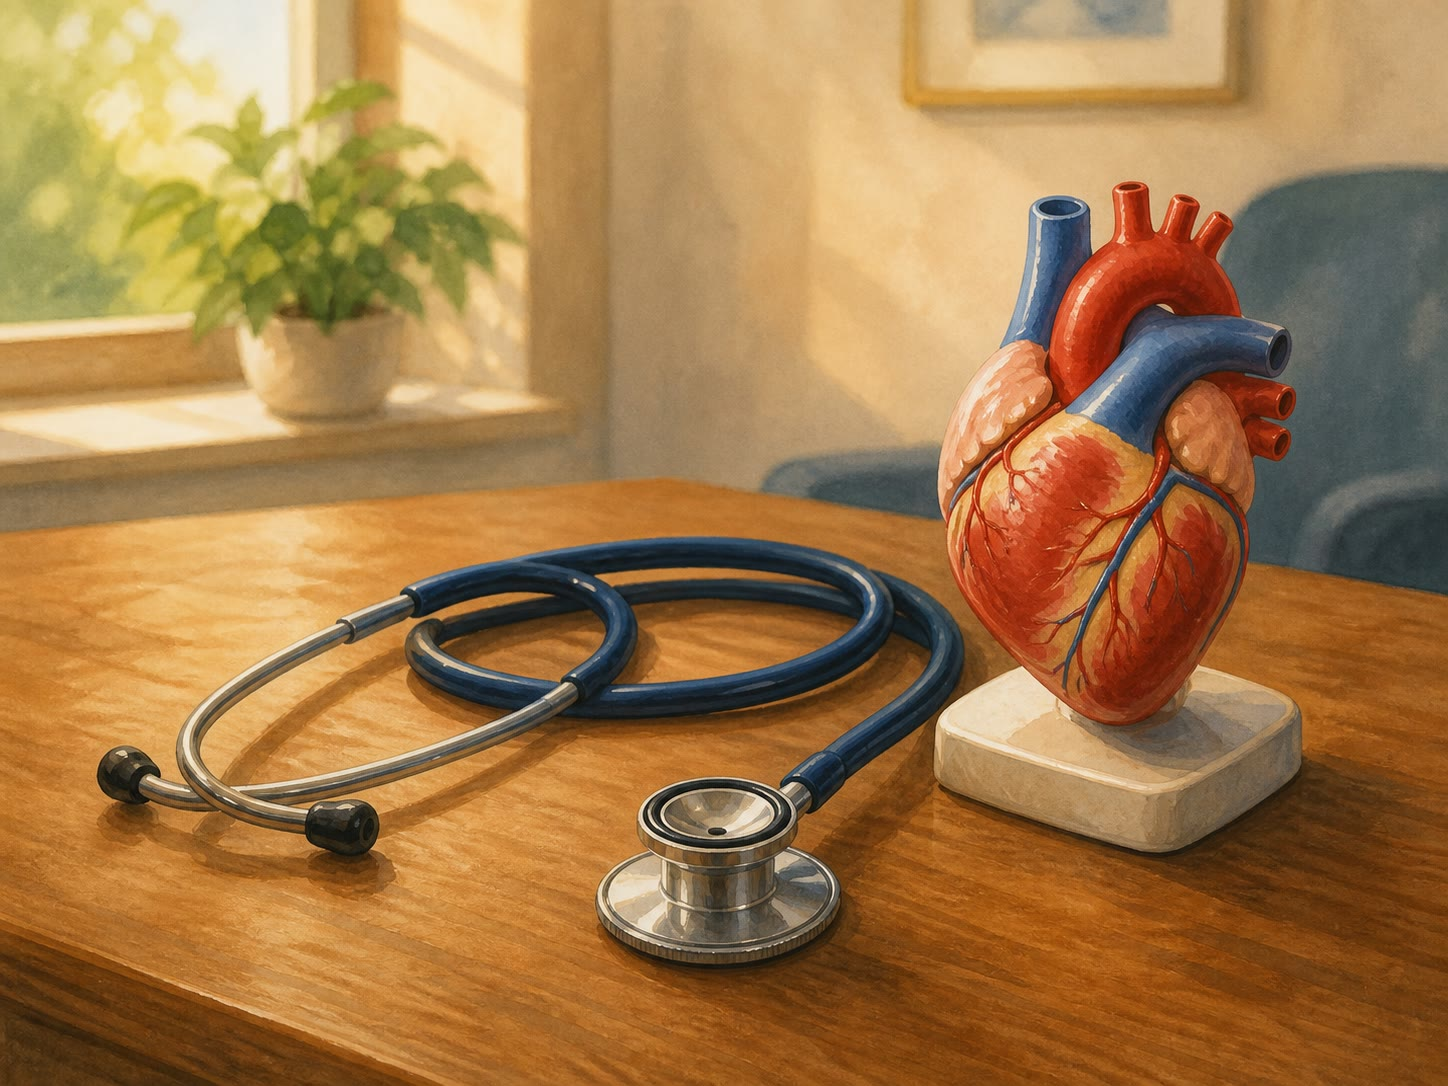
\includegraphics[width=0.56\linewidth]{images/book1/ai/g7-heart-stethoscope.jpg}

{\small Los dos clásicos de la consulta: el modelo que enseña las
habitaciones y los \omterm{def:g4:heart-and-blood:vessels}{vasos}, y el fonendoscopio que oye cerrarse sus
puertas.}
\end{omfigure}

\begin{proposition}[Conservar la red]\label{prop:g7:heart-and-circulation:keep}
Se conocen los enemigos y los amigos de la red a largo plazo:
\begin{itemize}
  \item el \emph{ejercicio} fortalece la bomba
        (\cref{prop:g7:organs-at-work:training}) y mantiene flexibles
        las autopistas;
  \item la \emph{alimentación equilibrada}
        (\cref{met:g3:balanced-diet:check}) protege las paredes de las
        \omterm{def:g7:heart-and-circulation:vessels}{arterias}, que una \omterm{prop:g4:journey-of-food:absorb}{sangre} demasiado rica va incrustando y
        endureciendo poco a poco;
  \item el \emph{humo} ataca a los \omterm{def:g4:heart-and-blood:vessels}{vasos} además de a los \omterm{def:g7:how-animals-breathe:four}{pulmones}
        (\cref{prop:g7:lungs-and-gas-exchange:smoke}) ---
        estrechándolos, endureciéndolos y robando asientos;
  \item el suministro del propio \omterm{def:g4:heart-and-blood:heart}{corazón} --- se alimenta por \omterm{def:g7:heart-and-circulation:vessels}{arterias}
        pequeñas propias, no de la \omterm{prop:g4:journey-of-food:absorb}{sangre} de sus habitaciones ---
        depende de las tres cosas.
\end{itemize}
Los hábitos de la \cref{prop:g5:healthy-choices:contract} son, en
concreto, mantenimiento de los \omterm{def:g4:heart-and-blood:vessels}{vasos}.
\end{proposition}
\admitted

\begin{method}[Colocar cualquier órgano en la red]\label{met:g7:heart-and-circulation:map}
Para cualquier órgano con el que se encuentre este libro:
\begin{enumerate}
  \item colócalo en el circuito general: \omterm{def:g7:heart-and-circulation:vessels}{arteria} de entrada, \omterm{def:g7:heart-and-circulation:vessels}{vena} de
        salida, \omterm{def:g7:heart-and-circulation:vessels}{capilares} dentro;
  \item enumera lo que atraviesa las paredes de sus \omterm{def:g7:heart-and-circulation:vessels}{capilares}, hacia
        dentro y hacia fuera (\omterm{prop:g7:digestion-and-nutrients:absorption}{vellosidades}: \omterm{def:g7:digestion-and-nutrients:families}{nutrientes} hacia dentro;
        \omterm{def:g3:bones-and-muscles:muscle}{músculo}: combustible y \omterm{def:g7:what-is-respiration:respiration}{oxígeno} hacia dentro, \omterm{def:g7:what-is-respiration:respiration}{dióxido de carbono}
        hacia fuera; \omterm{def:g1:the-five-senses:sense}{piel}: calor hacia fuera);
  \item anota su conexión especial, si la tiene (la \omterm{prop:g4:journey-of-food:absorb}{sangre} del
        intestino pasa antes por el \omterm{prop:g7:digestion-and-nutrients:absorption}{hígado}; los \omterm{def:g7:how-animals-breathe:four}{pulmones} están en su
        propio circuito);
  \item comprueba los flujos con la tarea del órgano --- el esquema de
        la red debería volver a contar el capítulo de ese órgano.
\end{enumerate}
\end{method}

\section{Ejercicios}

\begin{exercise}[$\star$]\label{exo:g7:heart-and-circulation:1}
Nombra las cuatro habitaciones del \omterm{def:g4:heart-and-blood:heart}{corazón} y el papel de cada una.
\end{exercise}

\begin{exercise}[$\star$]\label{exo:g7:heart-and-circulation:2}
¿Para qué son las \omterm{def:g7:heart-and-circulation:rooms}{válvulas} del \omterm{def:g4:heart-and-blood:heart}{corazón} y qué es el pum-pum?
\end{exercise}

\begin{exercise}[$\star$]\label{exo:g7:heart-and-circulation:3}
Traza los dos circuitos, nombrando de cada uno el punto de partida, el
destino y el retorno.
\end{exercise}

\begin{exercise}[$\star$]\label{exo:g7:heart-and-circulation:4}
Da las tres clases de vaso con un rasgo de construcción y una tarea de
cada una.
\end{exercise}

\begin{exercise}[$\star$]\label{exo:g7:heart-and-circulation:5}
¿Por qué es el \omterm{def:g7:heart-and-circulation:rooms}{ventrículo} izquierdo la habitación de paredes más gruesas?
\end{exercise}

\begin{exercise}[$\star$]\label{exo:g7:heart-and-circulation:6}
¿Dónde --- en qué clase de vaso --- ocurren todos los intercambios del
cuerpo? Nombra los intercambios \omterm{def:g7:heart-and-circulation:vessels}{capilares} de tres órganos.
\end{exercise}

\begin{exercise}[$\star\star$]\label{exo:g7:heart-and-circulation:7}
Repite el \cref{ex:g7:heart-and-circulation:tour} para una gota que
sirve al \omterm{def:g5:brain-in-command:system}{cerebro} en vez de al muslo. ¿Qué toma y qué deja el
intercambio \omterm{def:g7:heart-and-circulation:vessels}{capilar} del \omterm{def:g5:brain-in-command:system}{cerebro}? (La
\cref{prop:g5:brain-in-command:protect} enumera sus apetitos.)
\end{exercise}

\begin{exercise}[$\star\star$]\label{exo:g7:heart-and-circulation:8}
El \omterm{prop:g4:heart-and-blood:pulse}{pulso} se nota en las \omterm{def:g7:heart-and-circulation:vessels}{arterias}, nunca en las \omterm{def:g7:heart-and-circulation:vessels}{venas}. Explícalo con la
construcción y con la presión de los dos \omterm{def:g4:heart-and-blood:vessels}{vasos}.
\end{exercise}

\begin{exercise}[$\star\star$]\label{exo:g7:heart-and-circulation:9}
Las \omterm{def:g7:heart-and-circulation:vessels}{venas} tienen \omterm{def:g7:heart-and-circulation:rooms}{válvulas} de un solo sentido; las \omterm{def:g7:heart-and-circulation:vessels}{arterias} no. ¿Qué
problema resuelven las \omterm{def:g7:heart-and-circulation:rooms}{válvulas} de las \omterm{def:g7:heart-and-circulation:vessels}{venas} --- y por qué se desmayan
a veces los soldados que están firmes y quietos?
\end{exercise}

\begin{exercise}[$\star\star$]\label{exo:g7:heart-and-circulation:10}
Aplícale el \cref{met:g7:heart-and-circulation:map} al \omterm{def:g4:journey-of-food:tract}{intestino
delgado}, con su conexión especial incluida.
\end{exercise}

\begin{exercise}[$\star\star$]\label{exo:g7:heart-and-circulation:11}
¿Por qué necesita el \omterm{def:g4:heart-and-blood:heart}{corazón} sus propias \omterm{def:g7:heart-and-circulation:vessels}{arterias} pequeñas de
alimentación, con sus habitaciones llenas de \omterm{prop:g4:journey-of-food:absorb}{sangre}? ¿Y por qué importa
tanto que se incrusten?
\end{exercise}

\begin{exercise}[$\star\star\star$]\label{exo:g7:heart-and-circulation:12}
``El \omterm{def:g4:heart-and-blood:heart}{corazón} es fontanería al servicio de los \omterm{def:g7:heart-and-circulation:vessels}{capilares}''. Defiende la
afirmación con la \cref{rem:g7:heart-and-circulation:capillaries} y con
dos intercambios de capítulos anteriores.
\end{exercise}

\section{Problema: La mañana del cardiólogo}

\begin{problem}[{Problema de fin de semana --- cuatro consultas, un
mapa de la red}]\label{pb:g7:heart-and-circulation:1}
Acompaña a un cardiólogo durante una mañana de cuatro consultas
(inventadas), con el mapa en la mano.

\medskip\noindent\textbf{Parte I --- La referencia sana.}
\begin{enumerate}
  \item A la paciente 1, una \omterm{def:g3:stages-of-life:stages}{adolescente} en forma, le hacen las tres
        lecturas a pie de carretera del
        \cref{ex:g7:heart-and-circulation:measures}. Nombra cada una y
        qué parte de la maquinaria lee.
  \item Su \omterm{prop:g4:heart-and-blood:pulse}{pulso} en reposo es de $58$. El cardiólogo sonríe. ¿Por qué
        (\cref{exo:g4:heart-and-blood:11})?
  \item Su pum-pum es nítido y doble. ¿Qué se cerró de golpe,
        exactamente, dos veces en cada \omterm{def:g4:heart-and-blood:heart}{latido}?
  \item Esboza el camino de su \omterm{prop:g4:journey-of-food:absorb}{sangre} desde la \omterm{def:g7:heart-and-circulation:rooms}{aurícula} derecha por los
        dos circuitos y de vuelta, en ocho paradas con nombre.
\end{enumerate}

\medskip\noindent\textbf{Parte II --- Tres problemas.}
\begin{enumerate}[resume]
  \item El paciente 2 tiene una válvula que pierde entre la \omterm{def:g7:heart-and-circulation:rooms}{aurícula} y
        el \omterm{def:g7:heart-and-circulation:rooms}{ventrículo} izquierdos: en cada \omterm{def:g4:heart-and-blood:heart}{latido}, parte de la \omterm{prop:g4:journey-of-food:absorb}{sangre} se
        va hacia atrás, con un soplo silbante. Predice las
        consecuencias para las entregas del circuito general y para el
        aguante del paciente.
  \item El paciente 3, gran fumador y de dieta rica, tiene las \omterm{def:g7:heart-and-circulation:vessels}{arterias}
        incrustadas y endurecidas. ¿Qué lecturas de la consulta 1
        habrán empeorado y por qué trabaja horas extra el \omterm{def:g7:heart-and-circulation:rooms}{ventrículo}
        izquierdo?
  \item Las incrustaciones del paciente 3 incluyen las \omterm{def:g7:heart-and-circulation:vessels}{arterias} de
        alimentación del propio \omterm{def:g4:heart-and-blood:heart}{corazón}. Explica en una frase la
        preocupación especial del cardiólogo.
  \item La paciente 4 tiene los \omterm{def:g1:my-body:joint}{tobillos} hinchados después de días
        largos de pie: el retorno cuesta arriba de las \omterm{def:g7:heart-and-circulation:vessels}{venas} va con
        apuros. ¿Qué estructuras están fallando y por qué la alivia
        andar --- con los gemelos apretando las \omterm{def:g7:heart-and-circulation:vessels}{venas}?
\end{enumerate}

\medskip\noindent\textbf{Parte III --- El cartel de la pared.}
\begin{enumerate}[resume]
  \item El cartel de la consulta enseña el doble bucle. Explícale a un
        paciente que espera por qué la \omterm{prop:g4:journey-of-food:absorb}{sangre} tiene que visitar los
        \omterm{def:g7:how-animals-breathe:four}{pulmones} entre cada dos recorridos del cuerpo.
  \item Añade la leyenda de los \omterm{def:g4:heart-and-blood:vessels}{vasos}: \omterm{def:g7:heart-and-circulation:vessels}{arteria}, \omterm{def:g7:heart-and-circulation:vessels}{capilar}, \omterm{def:g7:heart-and-circulation:vessels}{vena} --- una
        línea de cada uno sobre construcción, presión y tarea.
  \item El pie del cartel dice: ``todo tratamiento está al servicio de
        los \omterm{def:g7:heart-and-circulation:vessels}{capilares}''. Justifícalo con la
        \cref{rem:g7:heart-and-circulation:capillaries}.
  \item Cierra la mañana con la receta de prevención que el cardiólogo
        le da a cada paciente --- tres hábitos, cada uno atado a su
        mecanismo en la \cref{prop:g7:heart-and-circulation:keep}.
\end{enumerate}
\end{problem}
